\chapter{Построение фрагмента онтологии теоретико-графовой задачи}

В этом разделе я описываю выполнение второго этапа расчетной
работы на примере задачи поиска минимального пути в неориентированном
графе. Для понимания руководства студент должен обладать следующими
знаниями: 

\begin{itemize}
\item базовые знания по теории графов
\item SC-коде и SC-алфавите
\item базовые знания о SCg-коде
\item уметь различать абсолютные и относительные понятия
\item знание правил формирования идентификаторов sc-элементов
\end{itemize}

\section{Задание}

Конечно, во-первых, что должны сделать вы, студент, при выполнении
этого этапа расчетной работы, это выделить абсолютные и относительные
понятия своей теоретико-графовой задачи. Список понятий должен
включать не только непосредственно необходимые для решения вашей
задачи, но и те понятия, на основе которых определены непосредственно
необходимые. Таким образом, будет выделена целая иерархия понятий.

Во-вторых, для каждого понятия разработать способ представления его
экземпляров в SC-коде. После этого необходимо показать отчет в
электронном варианте о проделанной работе, который должен содержать
следующее:

\begin{enumerate}
\item Перечень выделенных понятий со следующей информацией:
  \begin{enumerate}
  \item Название понятия;
  \item Абсолютное или относительное;
  \item Определение на естественном языке (его стоит брать из соответствующей
    литературы);
  \item Пример представления экземпляра понятия в SC-коде на
    SCg (не маленький и не большой, среднего размера). 
  \end{enumerate}
\item Пять примеров на SCg входных и выходных для вашей программы. 
\end{enumerate}

От первого к последнему примеры должны усложняться, и они должны быть
разнообразны, потому что в дальнейшем будут использоваться в качестве
тестов программы. В каждом примере должна быть показана какая-то
особенность задачи. В этом пункте можно использовать сокращенную форму
записи графов. Примеры нужно брать из предыдущего этапа расчетной
работы.

Стоит сказать несколько слов о списке понятий с определениями. Если вы
будете использовать понятия, описанные в этом руководстве, то в списке
достаточно привести только имя понятия и указать его тип (абсолютное
или относительное). Если вы будете брать понятия из базы знаний OSTIS
GT или самостоятельно выделять на основе литературы по теории графов,
то обязательно их описывать по полной форме.

Для рисования SCg-текстов необходимо использовать редактор KBE
(Knowledge Base Editor). Установщик и zip-архив собранной версии под
Windows можно найти в той же папке на сервере Info, откуда вы взяли
этот документ.

Мы плавно переходим к примеру выполнения 2-го этапа…

Выполненный мною пример отчета по этому этапу в docx-формате можно
найти в папке расчетной работы на сервере Info либо в конце этого
документа.  Напомню, что мы рассматриваем задачу поиска одного из
минимальных путей в неориентированном графе. Поэтому первым, чем мы
займемся, будет способ представления в SC-коде неориентированных
графов.


\section{Формализация понятия неориентированный граф}

На данном этапе выполнения расчетной работы для нас пока что неважен
собственно алгоритм решения теоретико-графовой задачи, а важны только
обрабатываемые данные (входные и выходные данные для
программы). Напомню, что мы рассматриваем задачу поиска одного из
минимальных путей в неориентированном графе. Поэтому первым, чем мы
займемся, будет способ представления в SC-коде неориентированных
графов.  

Возьмем для рассмотрения неориентированный граф $G$:

\begin{figure}[h]
  \centering
  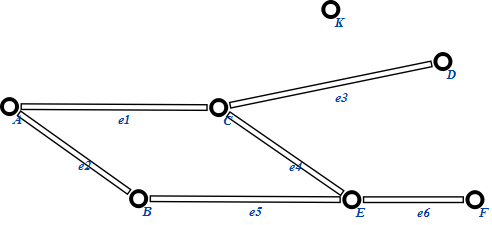
\includegraphics[scale=0.7]{images/2/Undirected_graph_not_scg}
  \caption{Неориентированный граф G (это не SCg)}
  \label{fig:Undirected_graph_not_scg}
\end{figure}

Распишем граф $G$ классическим способом на языке теории множеств:

\[ G = \langle V_g, E_g \rangle; \]
\[ V_g = \{A, B, C, E, D, F, K\}; \]
\[ E_g = \{\{A, B\}, \{A, C\}, \{C, E\}, \{C, D\}, \{B, E\}, \{E, F\}\}. \]

Теперь попробуем перевести запись, приведенную выше, в SC-код. Все
sc-конструкции я буду приводить на SCg. Для представления
неориентированного графа в SC-коде введем абсолютное понятие
неориентированный граф (это идентификатор sc-элемента; в дальнейшем я
буду использовать именно такое форматирования для идентификаторов в
тексте). Теперь мы можем преобразовать запись на языке теории
множеств, задающую граф G, в SCg-конструкцию:

\begin{figure}[h]
  \centering
  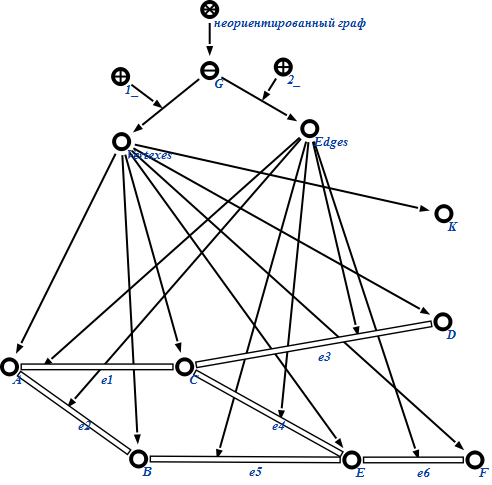
\includegraphics[scale=0.6]{images/2/Undirected_graph_Classical_method}
  \caption{Классический способ задания неориентированного графа G на SCg}
  \label{fig:Undirected_graph_Classical_method}
\end{figure}

Приведенный выше способ задания графа на языке классической теории
множеств является распространённым, но мы, с использованием SC-кода,
можем найти другую форму, так как имеем возможность задавать ролевые
отношения. Поэтому введем два относительных понятия (ролевых
отношения): вершина\_ и ребро\_. Тогда можно сформулировать, что
неориентированный граф задается множеством объектов, в котором объект
с ролью вершина\_ является вершиной графа, а объект с ролью ребро\_ -
ребром графа. На языке теории множеств, расширенном возможностью
задавать атрибуты (роли) у элементов кортежа, граф G будет задаваться
следующим выражением: 

\begin{eqnarray*}
  G &=& \langle вершина\_: A, вершина\_: B, вершина\_: C, \\
  && вершина\_: E, вершина\_: D, вершина\_: F, вершина\_: K, \\
  && ребро\_: \{A, B\}, ребро\_: \{A, C\}, ребро\_: \{C, E\}, \\
  && ребро\_: \{C, D\}, ребро\_: \{B, E\}, ребро\_: \{E, F\} \rangle.
\end{eqnarray*}

Тогда наш граф на SCg-языке будет записываться так:

\begin{figure}[h]
  \centering
  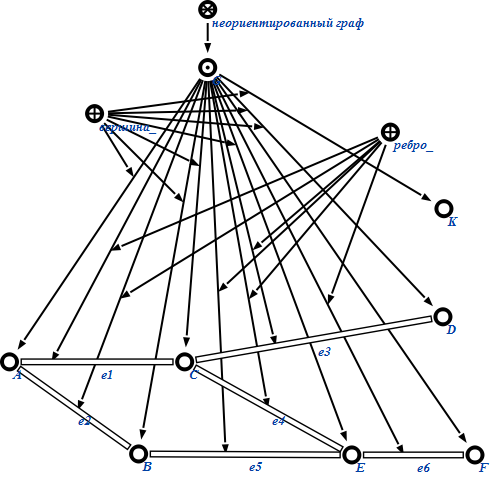
\includegraphics[scale=0.6]{images/2/Undirected_graph_Main_method}
  \caption{Основной для нас способ задания графа G на SCg}
  \label{fig:Undirected_graph_Main_method}
\end{figure}

Для студента, знакомого с теорией множеств и SCg-языком, в приведенном
выше рисунке необходимо пояснить только тип узла с идентификатором
G. Такой тип SCg-узла используется для обозначения sc-структуры,
т.е. множества объектов, которые могут выступать как целое. Объекты,
которые входят в sc-структуру, при совместном рассмотрении порождают
некоторое новое качество. Попробуем изучить это через сравнение
множества неориентированный граф с множеством G, которое является
конкретным неориентированным графом.  Множество неориентированный граф
– является sc-понятием (к слову, абсолютным) т.е. sc-множеством, все
элементы которого обладают некоторым заданным свойством. В случае
sc-понятия неориентированный граф его элементы должны обозначать
неориентированные графы. Количество элементов этого множества никогда
не переходит в качество. Совсем по-другому обстоят дела с множеством
G. Это sc-множество, составлено из sc-элементов, которые вместе
обладают некоторой целостностью, имеющей важные свойства (они образуют
неориентированный граф только в том случае, если рассмотрены как
единое целое). Такое sc-множество относится к абсолютному понятию
sc-структура.  Продолжая разговор о структурах, стоит сказать, что
связки так же являются структурами. Однако, очевидно, что
неориентированный граф G не только обозначает сам факт существования
связи между объектами, но и включает связки между своими собственными
элементами. Такие структуры, как граф G не являются связками, и мы
будем называть их одноуровневыми реляционными структурами.  Способ
представления графов в виде одноуровневых реляционных структур
используется в проекте базы знаний по теории графов технологии OSTIS
(OSTIS GT), поэтому ниже рассматривается только этот способ, и при
выполнении расчетной работы я рекомендую использовать именно
его. Продолжим рассмотрение того, как кодировать графы на sc-языках.
Давайте попробуем представить ориентированный граф на SCg. Преобразуем
неориентированный граф $G$ в ориентированный граф $G_d$:

\begin{figure}[h]
  \centering
  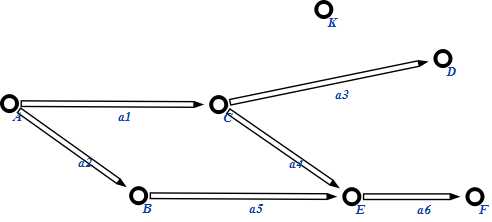
\includegraphics[scale=0.6]{images/2/Directed_graph_not_scg}
  \caption{Ориентированный граф $G_d$ (это не SCg)}
  \label{fig:Directed_graph_not_scg}
\end{figure}

Для представления $G_d$ на SCg введем абсолютное понятие ориентированный
граф и относительное понятие (ролевое отношение) дуга\_. С
использованием этих понятий граф $G_d$ на SCg можно представить
следующим образом:

\begin{figure}[h]
  \centering
  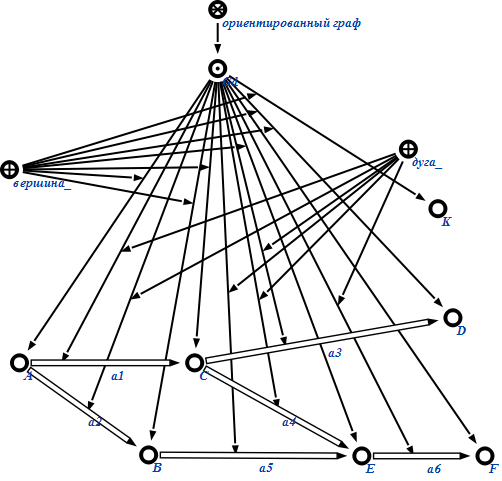
\includegraphics[scale=0.6]{images/2/Directed_graph}
  \caption{Ориентированный граф $G_d$ в SCg}
  \label{fig:Directed_graph}
\end{figure}

Сравните запись графа $G$ на SCg и графа $G_d$. Разница только в
использовании:

\begin{itemize}
\item узла ориентированный граф вместо неориентированный граф
\item узла дуга\_ вместо ребро\_
\item ориентированных бинарных пар вместо неориентированных
\end{itemize}

Можно заметить, что графы на SCg с использованием ролевых отношений
вершина\_ и ребро\_ получаются очень громоздкими, поэтому в дальнейших
объяснениях для представления неориентированных и ориентированных
графов мы будем использовать сокращенную запись. С использованием
сокращенной записи граф G, заданный на рис.
~\ref{fig:Undirected_graph_Main_method}, мы будем задавать так, как
показано на рис. ~\ref{fig:Undirected_graph_Short_form}. Надеюсь:
читатель понимает, что эта запись предназначена для понимания
человеком, а не машиной, потому что для машины является важным наличие
опущенных атрибутов (ролевых отношений).

\begin{figure}[h!]
  \centering
  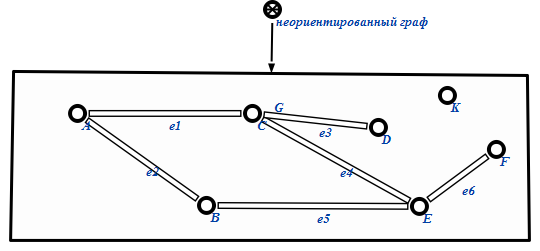
\includegraphics[scale=0.6]{images/2/Undirected_graph_Short_form}
  \caption{Сокращенная форма задbания графа $G$ на SCg Мы определились,}
  \label{fig:Undirected_graph_Short_form}
\end{figure}

Так будут кодироваться с использованием семантических
неориентированные и ориентированные графы. Теперь перейдем к
формализации минимального пути - второго понятия, без которого не
обойтись при решении нашей задачи.

\section{Формализация понятия минимального пути в SC-коде}

Если читатель заглянет в книгу (Харарри, 2003) на страницу 26, то в
начале главы <<Маршруты и связность>> он может прочитать следующее:


\begin{quotation}
  \textbf{Маршрутом} в графе $G$ называется чередующаяся
  последовательность вершин и ребер $v_0$, $x_1$, $v_1$, …, $v_{n-1}$,
  $x_n$, $v_n$; эта последовательность начинается и кончается
  вершиной, и каждое ребро последовательности инцидентно двум
  вершинам, одна из которых непосредственно предшествует ему, а другая
  непосредственно следует за ним. Указанный маршрут соединяет вершины
  $v_0$ и $v_n$, и его можно обозначить $v_0$, $v_1$, …, $v_n$
  (наличие ребер подразумевается).
\end{quotation}

Таким образом, минимальный путь — это маршрут, поэтому сейчас мы будем
рассматривать именно это более общее понятие. Если разберемся с
представлением его в SC-коде, то разберемся и с более частным
понятием.

Я думаю, что для читателя очевидно следующее: маршрут – это
относительное понятие, так как конкретный маршрут существует в связи с
конкретным графом. Поэтому для представления маршрутов введем бинарное
ориентированное отношение маршрут*. Первым компонентом связки этого
отношения будет знак графа, а вторым знак структуры маршрута. Пример
связки приведен на рис. \ref{fig:Example_of_relations_Route_tuple}.

\begin{figure}[h]
  \centering
  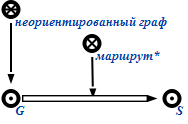
\includegraphics{images/2/Example_of_relations_Route_tuple}
  \caption{Пример связки отношения \idtf{маршрут*}}
  \label{fig:Example_of_relations_Route_tuple}
\end{figure}

Теперь нам необходимо выяснить из чего же состоит структура S на
рисунке \ref{fig:Example_of_relations_Route_tuple}. Для этого
рассмотрим в графе $G$ (рис. \ref{Undirected_graph_Short_form})
маршрут $R$ между вершинами $A$ и $F$, который задается последовательностью
$A$, $e_2$, $B$, $e_5$, $E$, $e_6$, $F$ (это один из минимальных путей между $A$ и
$F$). Если маршрут состоит из вершин и ребер, то маршрут можно
представить как подграф графа, на котором задается маршрут. Посмотрите
внимательно на риc. \ref{Route_as_subgraph}.

\begin{figure}
  \centering
  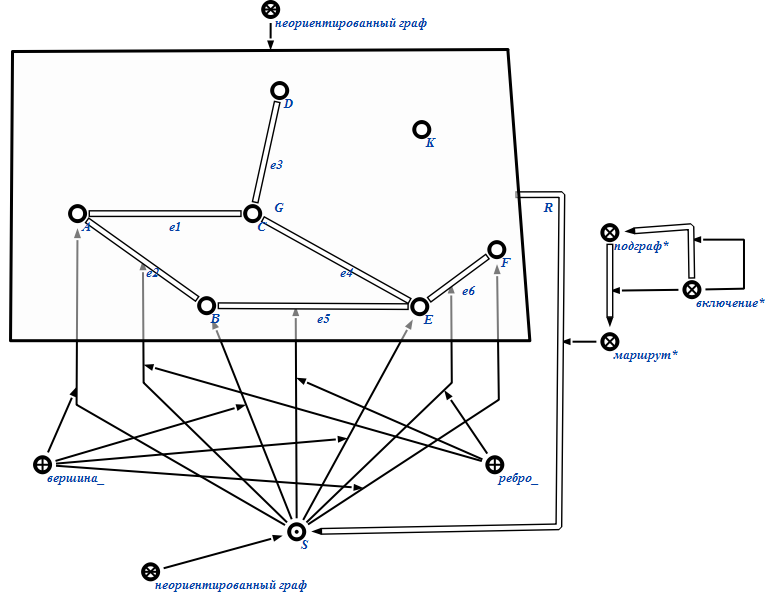
\includegraphics[scale=0.8]{images/2/Route_as_subgraph}
  \caption{Представление маршрута как подграфа графа $G$}
  \label{fig:Route_as_subgraph}
\end{figure}

Наверное, вы обратили внимание, что на рисунке появилось бинарное
ориентированное отношение \idtf{подграф*}, суть которого есть
связывание одного графа с другим графом, который является подграфом
первого. А еще из рисунка \ref{Route_as_subgraph} вы можете заметить,
что отношение \idtf{включение*} включает отношение \idtf{подграф*},
т.е. \idtf{подграф*} - аналог \idtf{включения*}, но только для
графов. А наше отношение \idtf{маршрут*} является подмножеством
отношения \idtf{подграф*}. Таким образом, граф структуры $S$ является
подграфом исходного графа $G$.

Возможно, вы посчитали, что на этом наш разговор о способе
представления маршрутов можно закончить, но я попрошу вас не
торопиться, а попробовать нарисовать SCg-конструкцию, которая задаст
маршрут $A$, $e_2$, $B$, $e_5$, $E$, $e_4$, $С$, $e_1$, $A$, $e_2$,
$B$. Ну как? Получилось? Хоть это и не путь, потому что вершины и
ребра повторяются, но это вполне допустимый маршрут. Если бы мне нужно
было объяснить вам, как написать просто еще одну программу, которая
находит минимальный путь в неориентированном графе, то такой способ
представления пути мне бы подошел. Но, на самом деле, моя задача
сейчас еще и показать вам, что надо найти такой наиболее общий способ
представления графов и маршрутов, чтобы для программ, которые решают
сходные задачи, не изобреталось что-то новое, а использовалось уже
разработанное представление. Тогда такие программы будут совместимы по
данным. Поэтому мы опять переходим к поиску способа задать структуру
второго компонента связки отношения \idtf{маршрут*} (структура $S$ на
рисунке \ref{fig:Example_of_relations_Route_tuple}).

Вернемся к тому, что мы решили рассматривать маршрут $R$ в графе
$G$. Тогда в основу нашего способа представления мы положили, что
маршрут состоит из вершин и ребер и он есть подграф графа, на котором
задается. Может быть, слабость этого подхода была в том, что мы не
рассматривали маршрут как последовательность вершин и ребер, т.е. мы
не задали порядок? Давайте попробуем задать последовательность
элементов маршрута.

Как мы можем задать последовательность? Если без введения лишних
понятий, то, например, при помощи ориентированного графа. Вершинами
такого графа будут элементы последовательности, а дуги будут задавать
отношение предыдущий/следующий. Первый элемент последовательности
специально указывать не будем, потому что первым элементом является
вершина, в которую нет входящих дуг. Последним элементом
последовательности будет вершина, из которой нет исходящих дуг. Этот
способ представления маршрута $R$ показан на рисунке 1.9.

\begin{figure}
  \centering
  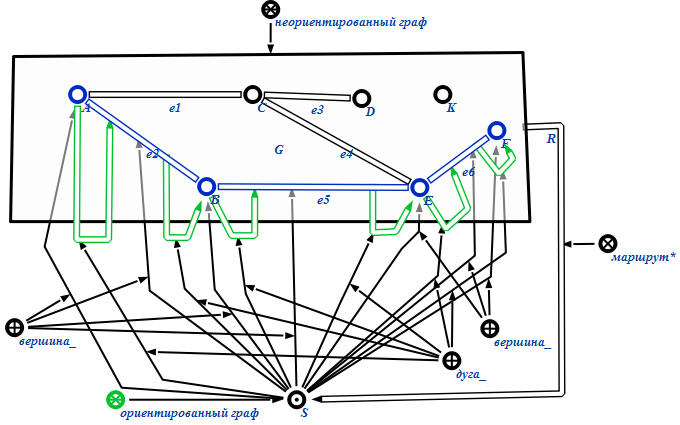
\includegraphics[scale=0.8]{images/2/Route_as_sequence}
  \caption{Представление маршрута через ориентированный граф последовательности}
  \label{fig:Route_as_sequence}
\end{figure}

Но, даже используя новый способ представления, мы не сможем задать
маршрут, который не является цепью или простой цепью (путем). Новый
способ представления все равно ограничен. Предлагаю вам увидеть это
самостоятельно, представив маршрут с повторяющимися вершинами и
ребрами. Поэтому продолжим наш поиск.

Давайте еще раз взглянем на определение маршрута из (Харарри, 2003):

\begin{quotation}
  \textbf{Маршрутом} в графе $G$ называется чередующаяся
  последовательность вершин и ребер $v_0$, $x_1$, $v_1$, …, $v_{n-1}$,
  $x_n$, $v_n$;
\end{quotation}

В нем сказано, что маршрут состоит из вершин и ребер. Но, быть может,
это не совсем так? Мы нашли два ограниченных способа для представления
маршрута, пользуясь буквально этим определением, а задачу еще не
решили. Может быть, стоит сказать, что маршрут состоит не из
последовательности вершин и ребер, а из последовательности посещений
вершин и ребер. Давайте попробуем использовать именно такую точку
зрения. Тогда мы можем преобразовать ориентированный граф
последовательности $S$ из рисунка \ref{fig:Route_as_sequence} в
ориентированный граф посещений $S$ на рисунке
\ref{fig:Route_as_correspondence_Incomplete}. Вершина графа $S$ на
рисунке \ref{fig:Route_as_correspondence_Incomplete} обозначает
посещение вершины графа $G$, а дуга графа $S$ – посещение ребра графа
$G$.

\begin{figure}
  \centering
  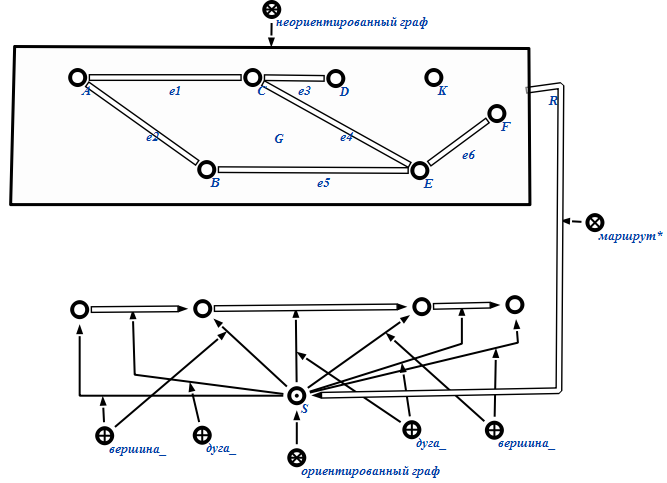
\includegraphics[scale=0.8]{images/2/Route_as_correspondence_Incomplete}
  \caption{Представление структуры $S$ маршрута $R$ как ориентированного графа посещений}
  \label{fig:Route_as_correspondence_Incomplete}
\end{figure}

На рисунке \ref{fig:Route_as_correspondence_Incomplete} не хватает
только связей между элементами посещения из графа $S$ и посещенными
элементами из графа $G$. Для того, чтобы мы могли закончить
конструкцию на рисунке \ref{fig:Route_as_correspondence_Incomplete},
вам надо вспомнить, что такое соответствие между двумя множествами, а,
если вы этого не знаете, то устранить пробел в вашем образовании. А
тем временем мы введем относительное понятие (тернарное отношение)
\idtf{соответствие*}, связка которого включает следующие три
компонента (пример связки на рисунке 1.11):

\begin{enumerate}
\item Множество, которое является областью определения соответствия
  (множество $X$ на рисунке 1.11).
\item Множество, которое является областью значений соответствия
  (множество $Y$ на рисунке 1.11).
\item Бинарное ориентированное отношение, которое устанавливает
  соответствие между элементом из области определения и элементом из
  области значения (отношение $Cr*$ на рисунке 1.11).
\end{enumerate}

\begin{figure}[h!]
  \centering
  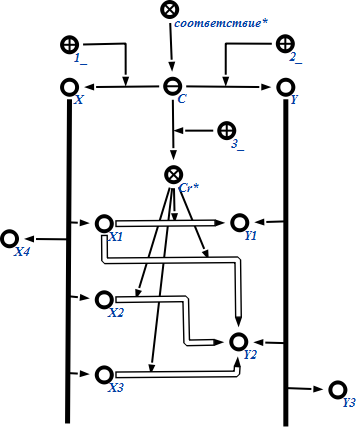
\includegraphics[scale=0.8]{images/2/Relation_Correspondence_example}
  \caption{Пример связки C отношения \idtf{соответствие*} между
    множествами $X$ и $Y$}
  \label{fig:Relation_Correspondence_example}
\end{figure}

Мы можем рассматривать маршрут $R$ как всюду определенное,
функциональное соответствие между ориентированным графом (структурой
маршрута) $S$ и неориентированным исходным графом $G$.  Тогда на
основе рисунков \ref{fig:Route_as_correspondence_Incomplete} и
\ref{fig:Relation_Correspondence_example} построим окончательный
вариант представления маршрута $R$ (рисунок
\ref{fig:Route_as_correspondence_Final}). Рассмотрим отличия
конструкции на рисунке \ref{fig:Route_as_correspondence_Final} от
конструкции на рисунке \ref{fig:Route_as_correspondence_Incomplete}:

\begin{enumerate}
\item Для наглядности упрощен ориентированный граф $S$ (скрыты узлы
  \attr{вершина} и \attr{дуга}).
\item Показано, что отношение \rel{маршрут} является подмножеством
  отношения \rel{соответствие}.
\item В связке $R$ первым компонентом теперь является граф $S$, а
  вторым – граф $G$. На рисунке
  \ref{fig:Route_as_correspondence_Incomplete} было наоборот. Чтобы
  понять, почему связка оказалась перевернутой, взгляните, пожалуйста,
  на рисунок \ref{fig:Relation_Correspondence_example}. На нем видно,
  что первым компонентом связки отношения \rel{соответствие} должно
  быть множество, которое является областью определения, а вторым –
  множество, которое является областью значения. Именно поэтому
  произошла такая перестановка.
\item Появилось отношения (третий компонент связки $R$), которое задает
  соответствие между посещением и посещенным элементом. Обратите
  внимание на направление бинарных ориентированных пар этого
  отношения!
\end{enumerate}

\begin{figure}[h!]
  \centering
  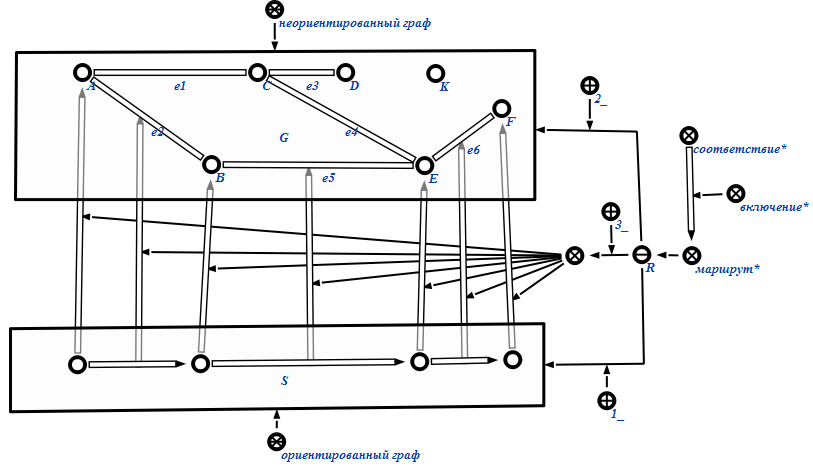
\includegraphics[scale=0.6]{images/2/Route_as_correspondence_Final}
  \caption{Окончательный вариант представления маршрута $R$, как
    соответствия между графом $S$ и графом $G$}
  \label{fig:Route_as_correspondence_Final}
\end{figure}

Попробуйте представить при помощи найденного нами способа (рисунок
\ref{fig:Route_as_correspondence_Final}) маршрут, в котором есть
повторяющиеся вершина и/или ребра. Я думаю, что теперь с этим у вас не
возникнет проблем. Подводя к концу разговор о способе представления
маршрутов в графе, введем относительные понятия (бинарные
ориентированные отношения) \rel{цепь} и \rel{путь}, которые связаны с
отношением \rel{маршрут} так, как показано на рисунке 1.13.

\begin{figure}[h!]
  \centering
  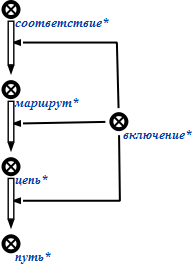
\includegraphics[scale=0.8]{images/2/Relations_Trail_and_Path}
  \caption{Связь отношений \rel{цепь} и \rel{путь} с отношением
    \rel{маршрут}}
  \label{fig:Relations_Trail_and_Path}
\end{figure}

Тогда один из минимальных путей $R$ ($A$, $e_2$, $B$, $e_5$, $E$,
$e_6$, $F$) в графе $G$ между вершинами A и F будет представляться в
SC-коде так, как показано на рисунке \ref{fig:Path_Final}. Правда,
несильно отличается от рисунка
\ref{fig:Route_as_correspondence_Final}?

\begin{figure}[h!]
  \centering
  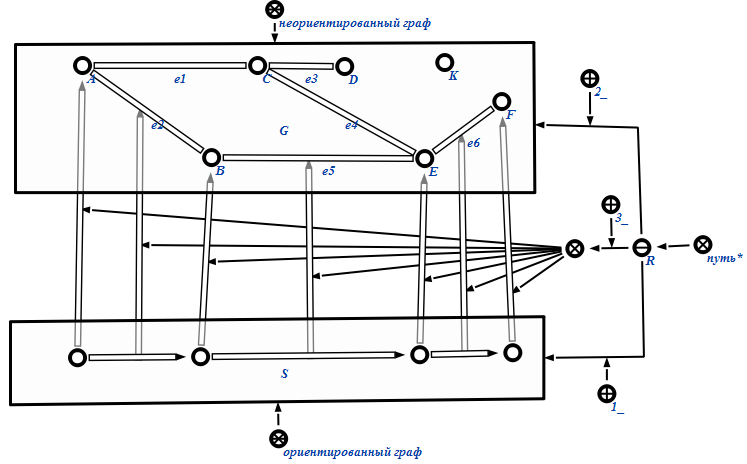
\includegraphics[scale=0.6]{images/2/Path_Final}
  \caption{Один из минимальных путей R между вершинами А и F графа G}
  \label{fig:Path_Final}
\end{figure}
 
На этом мы заканчиваем разговор о минимальном пути и переходим к
разговору о том, как можно обобщить представление различных видов
графов в SC-коде.

\section{Обобщение различных видов графов с использованием понятия графовой структуры}

В предыдущем разделе, когда мы искали способ представления
минимального пути в SC-коде, то сосредоточились на представлении
наиболее общего понятия по отношению к понятию путь, а именно –
маршрута. Таким образом, определившись с кодированием понятия
\rel{маршрут}, мы определились и с кодированием понятия \rel{путь}. А
вот, когда мы разбирались с неориентированными и ориентированными
графами, то рассматривали только то, что необходимо для решения нашей
задачи, игнорируя более общие случаи. Теперь пришло время посмотреть
на задачу представления графов в SC-коде более широко. Для этого мы
обратимся к базе знаний по теории графов из проекта OSTIS GT. Неполная
иерархия различных типов графов из этой базы знаний изображена на
рисунке 1.15. Я думаю, что вы уже заметили узлы ориентированный граф и
неориентированный граф. Однако они составляют только «низ» иерархии,
так как определены на основе более общих понятий. А начнем
рассматривать иерархию с «верха», а именно, с понятия графовая
структура.

\begin{figure}[h!]
  \centering
  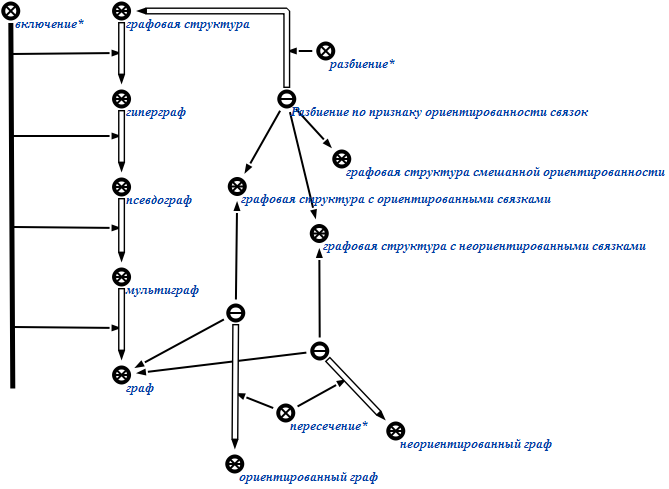
\includegraphics[scale=0.7]{images/2/Hierarchy_of_graphs_types}
  \caption{Иерархия различных типов графовых структур (Это неполная
    иерархия из OSTIS GT)}
  \label{fig:Hierarchy_of_graphs_types}
\end{figure}

Экземпляр понятия графовая структура – это такая одноуровневая реляционная структура, которая содержит объекты с ролью вершина_, а связки между этими объектами - с ролью связка_. Вроде бы по определению графовая структура несильно отличается от неориентированного графа. Взяли просто и заменили ролевое отношение ребро_ на связка_. И вот тут есть один нюанс. На элементы с ролью связка_ графовой структуры не накладывается ограничений, как на элементы с ролью ребро_ неориентированного графа, а именно:
1.	Они могут быть любой арности, а не только бинарными.
2.	Они могут быть как ориентированными, так и неориентированными.
3.	Их компонентами могут быть не только вершины, но и другие связки (т.е. разрешены связки, «выходящие» из связок, и связки, входящие в другие связки).
На рисунке 1.16 приведен пример графовой структуры Gs, в которой четыре вершины и три связки. Я хочу отметить, что графовая структура вполне может включать элементы с ролью ребро_. Просто связка_ более общее понятие, чем ребро_. Чтобы лучше увидеть связь между этими ролевыми отношениями, рассмотрите рисунок 1.17, на котором изображена иерархия ролевых отношений элементов графовой структуры из базы знаний по теории графов. А после того, как закончите, мы перейдем к краткому описанию абсолютных понятий гиперграф, псевдограф, мультиграф и граф.
 
1.16 Пример графовой структуры Gs
 
Рисунок 1.17 Иерархия ролей элементов графовой структуры (Это неполная иерархия из OSTIS GT)
Экземпляр понятия гиперграф (см. рисунок 1.15) – это такая графовая структура, в которой элемент с ролью связка_ может иметь в качестве своих компонентов только элемент с ролью вершина_ этой графовой структуры.  На арность связок никакого ограничения не накладывается. Для указания связки введены ролевые отношения гиперсвязка_, гипердуга_, гиперребро_ (рисунок 1.17). Обратите внимание на то, что на рисунке 1.17 гипердуга_ определена как пересечение понятий гиперсвязка_ и ориентированная дуга_. Аналогично дела обстоят с понятием гиперребро_. Пожалуйста, обдумайте самостоятельно такой способ введения новых понятий.
Экземпляр понятия псевдограф (см. рисунок 1.15) – это такой гиперграф, в котором гиперсвязка может иметь только два компонента.  Для указания связки введены ролевые отношения бинарная связка_, петля_, дуга_, ребро_ (рисунок 1.17). Петлей называется бинарная связка, у которой оба компонента одинаковы.
Экземпляр понятия мультиграф (см. рисунок 1.15) – это такой псевдограф, в котором не может быть петель. 
Экземпляр понятия граф (см. рисунок 1.15) – это такой мультиграф, в котором не может быть кратных связок, т.е. связок у которых первый и второй компоненты совпадают. 
А теперь самостоятельно на основе рисунка 1.15 рассмотрите то, как определены уже знакомые вам понятия ориентированный граф и неориентированный граф. На этом закончим пояснительную часть данного этапа и перейдем к более конкретной формулировке задания. 

\section{Пример выполнения}

\subsection{Список понятий}

\begin{itemize}
\item Графовая структура (абсолютное понятие) - это такая
  одноуровневая реляционная структура, объекты которой могут играть
  роль либо вершины, либо связки:
  \begin{itemize}
  \item Вершина (относительное понятие, ролевое отношение);
  \item Связка (относительное понятие, ролевое отношение).
  \end{itemize}

  \begin{figure}[h!]
    \centering
    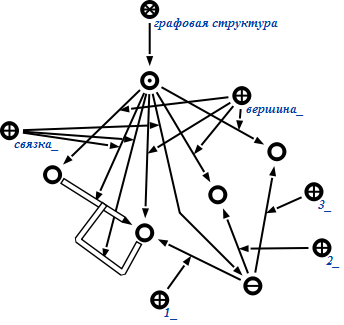
\includegraphics[scale=0.3]{images/2/concept/Graph_structure}
    \label{fig:Concept_Graph_structure}
  \end{figure}


\item Графовая структура с ориентированными связками (абсолютное
  понятие)
  \begin{itemize}
  \item Ориентированная связка (относительное понятие, ролевое
    отношение) – связка, которая задается ориентированным множеством.
  \end{itemize}

\item Графовая структура с неориентированными связками (абсолютное
  понятие)
  \begin{itemize}
  \item Неориентированная связка (относительное понятие, ролевое
    отношение) – связка, которая задается неориентированным
    множеством.
  \end{itemize}

\item Гиперграф (абсолютное понятие) – это такая графовая структура, в
  которой связки могут связывать только вершины:
  \begin{itemize}
  \item Гиперсвязка (относительное понятие, ролевое отношение);
  \item Гипердуга (относительное понятие, ролевое отношение) –
    ориентированная гиперсвязка;
  \item Гиперребро (относительное понятие, ролевое отношение) –
    неориентированная гиперсвязка.
  \end{itemize}

\item Псевдограф (абсолютное понятие) – это такой гиперграф, в котором
  все связки должны быть бинарными.
  \begin{itemize}
  \item Бинарная связка (относительное понятие, ролевое отношение)
    – гиперсвязка арности 2; 
  \item Ребро (относительное понятие, ролевое
    отношение) – неориентированная гиперсвязка;
  \item Дуга (относительное понятие, ролевое отношение) –
    ориентированная гиперсвязка;
  \item Петля (относительное понятие, ролевое отношение) – бинарная
    связка, у которой первый и второй компоненты совпадают.
  \end{itemize}

\item Мультиграф (абсолютное понятие) – это такой псевдограф, в
  котором не может быть петель.
 
\item Граф (абсолютное понятие) – это такой мультиграф, в котором не
  может быть кратных связок, т.е. связок у которых первый и второй
  компоненты совпадают.
 
\item Неориентированный граф (абсолютное понятие) – это такой граф, в
  котором все связки являются ребрами:
 
\item Ориентированный граф (абсолютное понятие) - это такой граф, в
  котором все связки являются дугами:
 
\item Маршрут (относительное понятие, бинарное ориентированное
  отношение) – это чередующаяся последовательность вершин и
  гиперсвязок в гиперграфе, которая начинается и кончается вершиной, и
  каждая гиперсвязка последовательности инцидентна двум вершинам, одна
  из которых непосредственно предшествует ей, а другая непосредственно
  следует за ней. В примере ниже показан маршрут $A$, $CON1$, $C$,
  $CON2$, $D$, $CON3$, $B$, $CON1$, $A$ в гиперграфе. Обратите внимание, что
  графы в примере приведены в сокращенной форме, что $CON1$ – это
  тернарная неориентированная связка (гиперсвязка), а $CON2$ и $CON3$ –
  бинарные связки (гиперсвязки).
 
\item Цепь (относительное понятие, бинарное ориентированное отношение)
  – это маршрут, все гиперсвязки которого различны. В примере ниже
  показана цепь $A$, $CON1$, $C$, $CON2$, $D$, $CON3$, $B$, $CON1$,
  $A$ в гиперграфе.
 
\item Простая цепь, путь (относительное понятие, бинарное
  ориентированное отношение) – это цепь, в которой все вершины
  различны. В примере ниже показан путь$A$, $CON1$, $C$, $CON2$, $D$,
  $CON3$, $B$ в гиперграфе.

\end{itemize}

\subsection{Тестовые примеры}

Во всех тестах графы будет приведены в сокращенной форме со скрытыми
ролями элементов графа.

\newpage

\subsubsection{Тест 1}
\textbf{Вход:}
Необходимо найти минимальный путь между вершинами $A$ и $C$. 

\begin{figure}[h!]
  \centering
  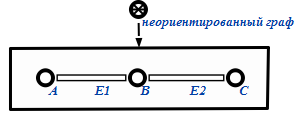
\includegraphics{images/2/test/1_In}
  \label{fig:Test1_In}
\end{figure}

\textbf{Выход:}
Будет найден единственный минимальный путь $A$, $E1$, $B$, $E2$, $C$:

\begin{figure}[h!]
  \centering
  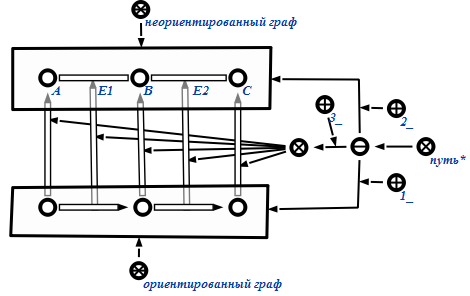
\includegraphics{images/2/test/1_Out}
  \label{fig:Test1_Out}
\end{figure}

\newpage

\subsubsection{Тест 2}
\textbf{Вход:}
Необходимо найти минимальный путь между вершинами $A$ и $F$.

\begin{figure}[h!]
  \centering
  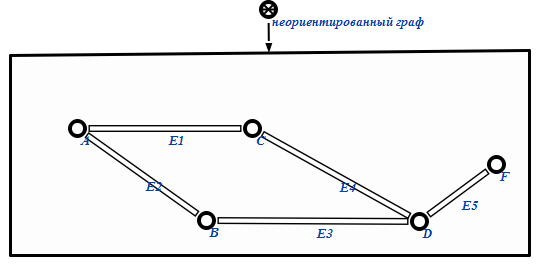
\includegraphics[scale=0.7]{images/2/test/2_In}
  \label{fig:Test2_In}
\end{figure}

\textbf{Выход:}
Будет найден один из двух минимальный путь $A$, $E2$, $B$, $E3$, $D$, $E5$, $F$:

\begin{figure}[h!]
  \centering
  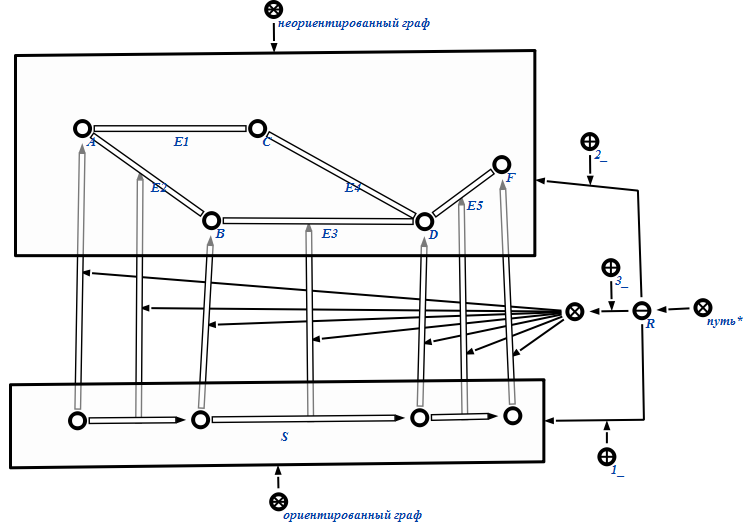
\includegraphics[scale=0.7]{images/2/test/2_Out}
  \label{fig:Test2_Out}
\end{figure}

\newpage

\subsubsection{Тест 3}
\textbf{Вход:}
Необходимо найти минимальный путь между вершинами $A$ и $K$. 

\begin{figure}[h!]
  \centering
  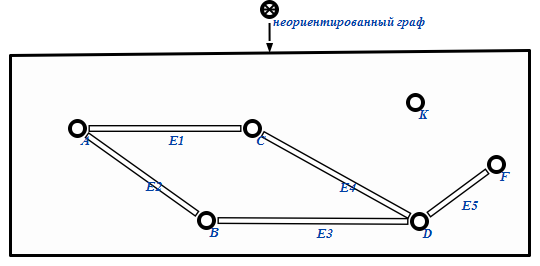
\includegraphics[scale=0.8]{images/2/test/3_In}
  \label{fig:Test3_In}
\end{figure}


\textbf{Выход:}
Минимального пути между вершинами $A$ и $K$ не существует. Программа должна вернуть ошибку вызывающему контексту.

\newpage

\subsubsection{Тест 4}
\textbf{Вход:}
Необходимо найти минимальный путь между вершинами $V5$ и $V11$. 

\begin{figure}[h!]
  \centering
  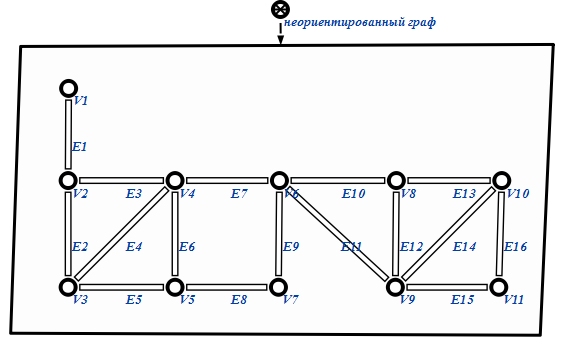
\includegraphics[scale=0.6]{images/2/test/4_In}
  \label{fig:Test4_In}
\end{figure}


\textbf{Выход:}
Будет найден один из двух минимальный путь $V5$, $E8$, $V7$, $E9$, $V6$, $E11$, $V9$, $E15$, $V11$:

\begin{figure}[h!]
  \centering
  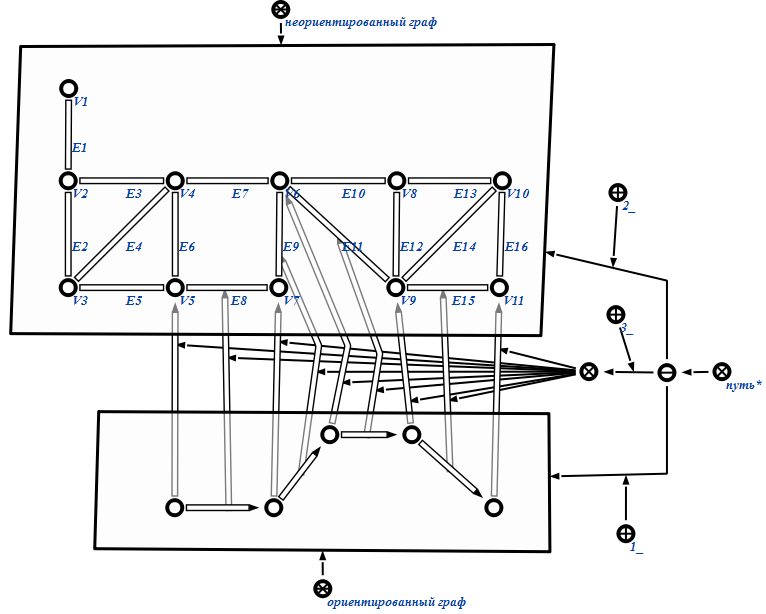
\includegraphics[scale=0.6]{images/2/test/4_Out}
  \label{fig:Test4_Out}
\end{figure}

\newpage

\subsubsection{Тест 5} 
\textbf{Вход:}
Необходимо найти минимальный путь между вершинами $V1$ и $V9$.

\begin{figure}[h!]
  \centering
  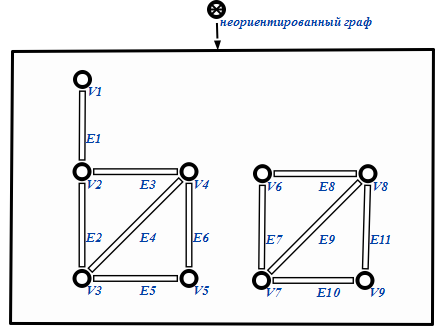
\includegraphics[scale=0.7]{images/2/test/5_In}
  \label{fig:Test5_In}
\end{figure}

 
\textbf{Выход:}
Минимального пути между вершинами $V1$ и $V9$ не существует. Программа должна вернуть ошибку вызывающему контексту.

%%% Local Variables: 
%%% mode: latex
%%% TeX-master: "main"
%%% End: 
